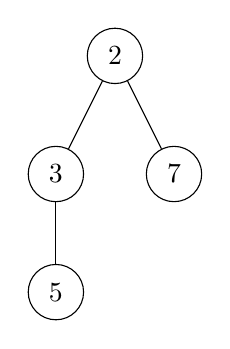
\begin{tikzpicture}
\node [shape=circle, minimum size = 2em, draw=black] (v3) at (3.75,0) {$2$};
\node [shape=circle, minimum size = 2em, draw=black] (v6) at (4.5,-1.5) {$7$};
\node [shape=circle, minimum size = 2em, draw=black] (v4) at (3,-1.5) {$3$};
\node [shape=circle, minimum size = 2em, draw=black] (v5) at (3,-3) {$5$};
\draw  (v3) edge (v4);
\draw  (v4) edge (v5);
\draw  (v3) edge (v6);
\end{tikzpicture}